% Überarbeitung von:
% NIT Patna Resume Template v2.1
% Author: Pavan Kumar Dubasi
% NIT Patna - IMSc., Mathematics (2019-24)
% LinkedIn: https://www.linkedin.com/in/im-pavankumar/
% 


\documentclass[a4paper,11pt]{article}

% Package imports
\usepackage{latexsym}
\usepackage{xcolor}
\usepackage{float}
\usepackage{ragged2e}
\usepackage[empty]{fullpage}
\usepackage{wrapfig}
\usepackage{tabularx}
\usepackage{titlesec}
\usepackage{geometry}
\usepackage{marvosym}
\usepackage{verbatim}
\usepackage{enumitem}
\usepackage{fancyhdr}
\usepackage{multicol}
\usepackage{graphicx}
\usepackage{cfr-lm}
\usepackage[T1]{fontenc}
\usepackage{fontawesome5}
\usepackage[hidelinks]{hyperref}
\usepackage{microtype}
\usepackage{tabularx} % Required for tables that stretch to page width
\usepackage{array} % Required for vertical centering in tables
% Color definitions
\definecolor{darkblue}{RGB}{0,0,139}

% Page layout
\geometry{left=1.4cm, top=0.8cm, right=1.2cm, bottom=1cm}
\setlength{\multicolsep}{0pt} 
\pagestyle{fancy}
\fancyhf{} % clear all header and footer fields
\fancyfoot{}
\renewcommand{\headrulewidth}{0pt}
\renewcommand{\footrulewidth}{0pt}
\setlength{\footskip}{4.08pt}

% Hyperlink setup
\hypersetup{
    colorlinks=true,
    linkcolor=darkblue,
    filecolor=darkblue,
    urlcolor=darkblue,
}

% Custom box settings
\usepackage[most]{tcolorbox}
\tcbset{
    frame code={},
    center title,
    left=0pt,
    right=0pt,
    top=0pt,
    bottom=0pt,
    colback=gray!20,
    colframe=white,
    width=\dimexpr\textwidth\relax,
    enlarge left by=-2mm,
    boxsep=4pt,
    arc=0pt,outer arc=0pt,
}

% URL style
\urlstyle{same}

% Text alignment
\raggedright
\setlength{\tabcolsep}{0in}

% Section formatting
\titleformat{\section}{
  \vspace{-4pt}\scshape\raggedright\large\bfseries
}{}{0em}{}[\color{black}\titlerule \vspace{-7pt}]

% Custom commands
\newcommand{\resumeItem}[2]{
  \item{
    \textbf{#1}{\hspace{0.5mm}#2 \vspace{-0.5mm}}
  }
}

\newcommand{\resumePOR}[3]{
\vspace{0.5mm}\item
    \begin{tabular*}{0.97\textwidth}[t]{l@{\extracolsep{\fill}}r}
        \textbf{#1}\hspace{0.3mm}#2 & \textit{\small{#3}} 
    \end{tabular*}
    \vspace{-2mm}
}

\newcommand{\resumeSubheading}[4]{
\vspace{0.5mm}\item
    \begin{tabular*}{0.98\textwidth}[t]{l@{\extracolsep{\fill}}r}
        \textbf{#1} & \textit{\footnotesize{#4}} \\
        \textit{\footnotesize{#3}} &  \footnotesize{#2}\\
    \end{tabular*}
    \vspace{-2.4mm}
}

\newcommand{\resumeProject}[4]{
\vspace{0.5mm}\item
    \begin{tabular*}{0.98\textwidth}[t]{l@{\extracolsep{\fill}}r}
        \textbf{#1} & \textit{\footnotesize{#3}} \\
        \footnotesize{\textit{#2}} & \footnotesize{#4}
    \end{tabular*}
    \vspace{-2.4mm}
}

\newcommand{\resumeSubItem}[2]{\resumeItem{#1}{#2}\vspace{-4pt}}

\renewcommand{\labelitemi}{$\vcenter{\hbox{\tiny$\bullet$}}$}
\renewcommand{\labelitemii}{$\vcenter{\hbox{\tiny$\circ$}}$}

\newcommand{\resumeSubHeadingListStart}{\begin{itemize}[leftmargin=*,labelsep=1mm]}
\newcommand{\resumeHeadingSkillStart}{\begin{itemize}[leftmargin=*,itemsep=1.7mm, rightmargin=2ex]}
\newcommand{\resumeItemListStart}{\begin{itemize}[leftmargin=*,labelsep=1mm,itemsep=0.5mm]}

\newcommand{\resumeSubHeadingListEnd}{\end{itemize}\vspace{2mm}}
\newcommand{\resumeHeadingSkillEnd}{\end{itemize}\vspace{-2mm}}
\newcommand{\resumeItemListEnd}{\end{itemize}\vspace{-2mm}}
\newcommand{\cvsection}[1]{%
\vspace{2mm}
\begin{tcolorbox}
    \textbf{\large #1}
\end{tcolorbox}
    \vspace{-4mm}
}

\newcolumntype{L}{>{\raggedright\arraybackslash}X}%
\newcolumntype{R}{>{\raggedleft\arraybackslash}X}%
\newcolumntype{C}{>{\centering\arraybackslash}X}%

% Commands for icon sizing and positioning
\newcommand{\socialicon}[1]{\raisebox{-0.05em}{\resizebox{!}{1em}{#1}}}
\newcommand{\ieeeicon}[1]{\raisebox{-0.3em}{\resizebox{!}{1.3em}{#1}}}

% Font options
\newcommand{\headerfonti}{\fontfamily{phv}\selectfont} % Helvetica-like (similar to Arial/Calibri)
\newcommand{\headerfontii}{\fontfamily{ptm}\selectfont} % Times-like (similar to Times New Roman)
\newcommand{\headerfontiii}{\fontfamily{ppl}\selectfont} % Palatino (elegant serif)
\newcommand{\headerfontiv}{\fontfamily{pbk}\selectfont} % Bookman (readable serif)
\newcommand{\headerfontv}{\fontfamily{pag}\selectfont} % Avant Garde-like (similar to Trebuchet MS)
\newcommand{\headerfontvi}{\fontfamily{cmss}\selectfont} % Computer Modern Sans Serif
\newcommand{\headerfontvii}{\fontfamily{qhv}\selectfont} % Quasi-Helvetica (another Arial/Calibri alternative)
\newcommand{\headerfontviii}{\fontfamily{qpl}\selectfont} % Quasi-Palatino (another elegant serif option)
\newcommand{\headerfontix}{\fontfamily{qtm}\selectfont} % Quasi-Times (another Times New Roman alternative)
\newcommand{\headerfontx}{\fontfamily{bch}\selectfont} % Charter (clean serif font)

% Define personal information
\newcommand{\name}{Leon Marquardt} % Your Name
\newcommand{\course}{} % Your Course
\newcommand{\roll}{} % Your Roll No.
\newcommand{\phone}{+49 160 94830980} % Your Phone Number
\newcommand{\emaila}{leon.marquardt@gmx.de} % Email 1
%\newcommand{\emailb}{officialemail@nitp.ac.in} % Email 2
\newcommand{\github}{lmarquar} % Github
\newcommand{\website}{blog.lmarquar.de} % Website
\newcommand{\gravatar}{leonmarquardt} % LinkedIn

\begin{document}
\fontfamily{cmr}\selectfont

%----------HEADING-----------------
\parbox{2.35cm}{%
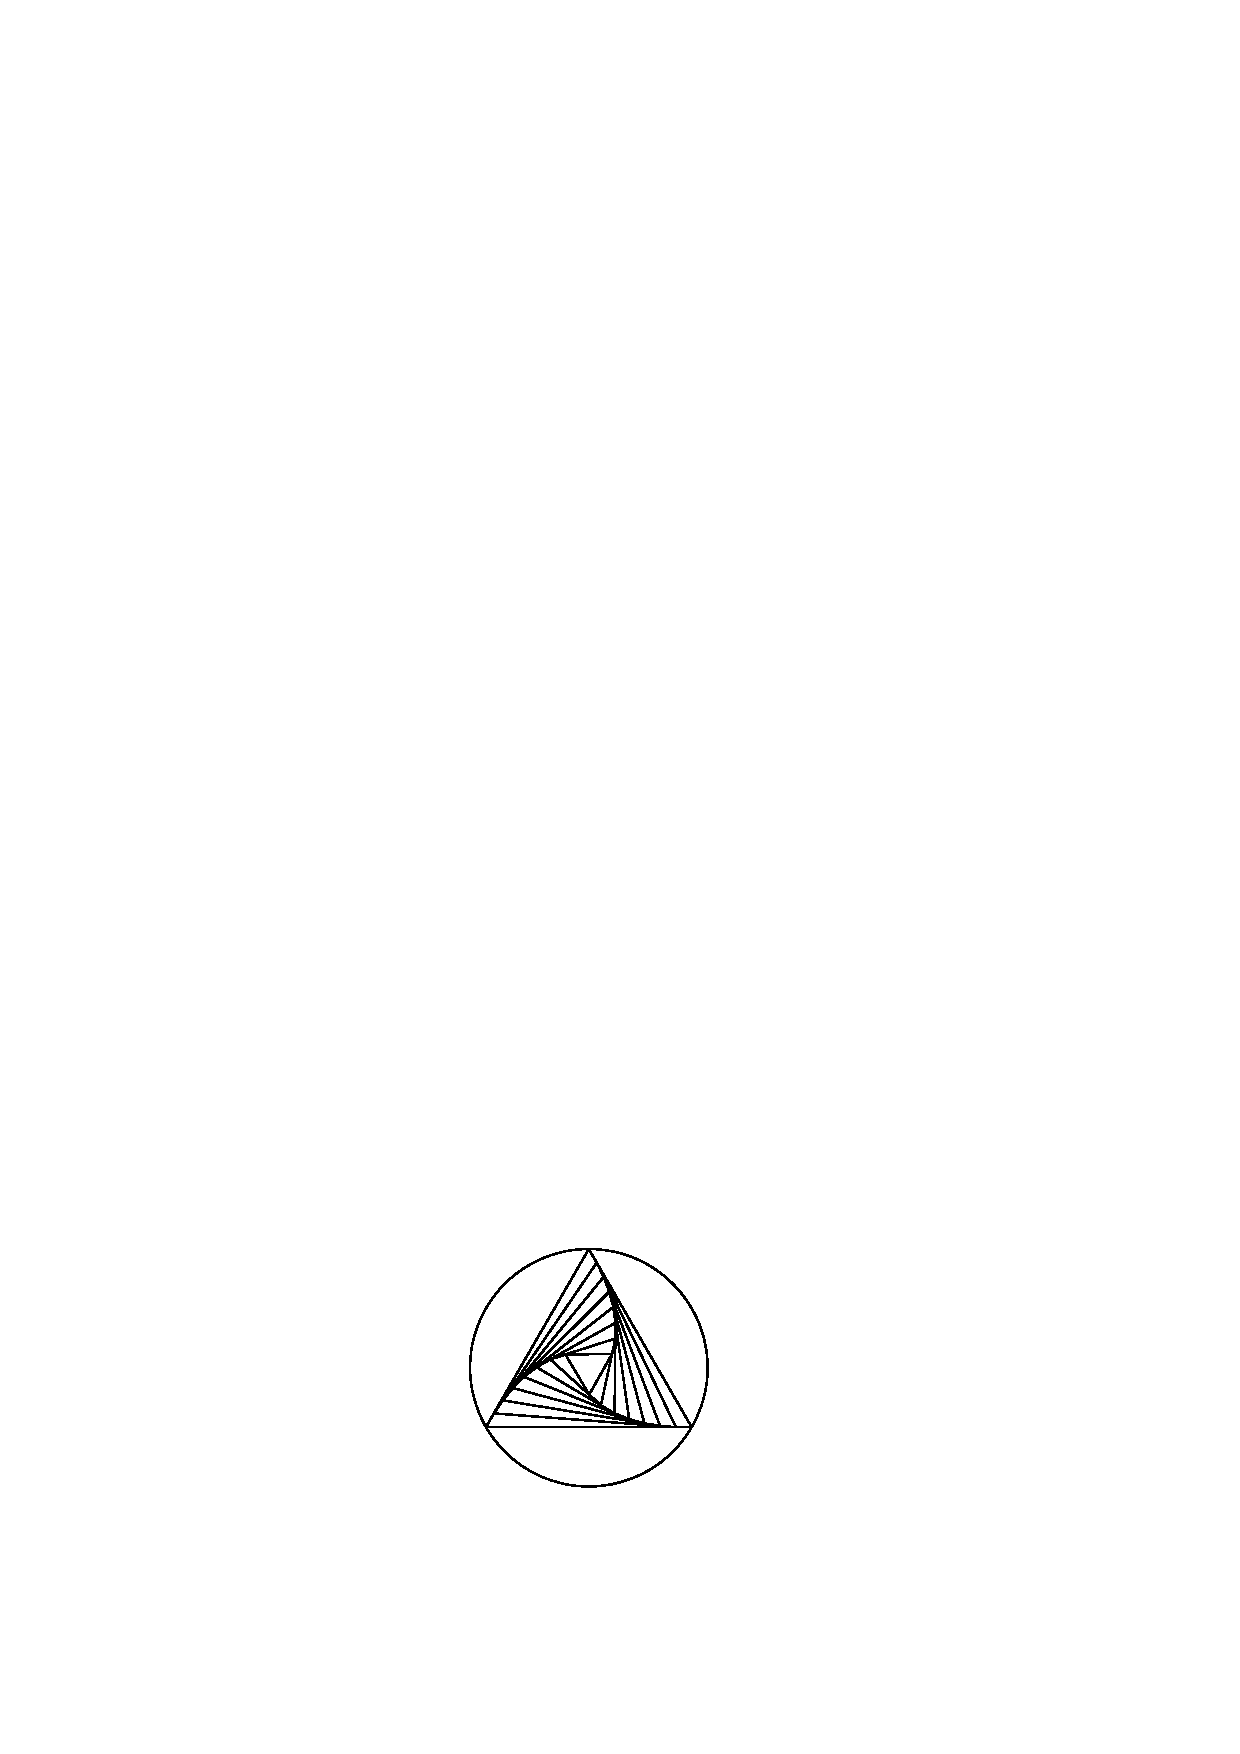
\includegraphics[trim=200 100 0 580, width=5cm]{Drawing1.pdf}
}
\parbox{\dimexpr\linewidth-2.8cm\relax}{
\begin{tabularx}{\linewidth}{L r}
  \textbf{\LARGE \name} & \phone \\
  \course & \href{mailto:\emaila}{\emaila} \\ & \href{https://gravatar.com/\gravatar}{gravatar.com/\gravatar} \\
\end{tabularx}
}
\vspace{-2mm}

\section{\textbf{Ausbildung}}
\vspace{1mm}
\setlength{\tabcolsep}{5pt}
\begin{tabularx}{\textwidth}{|>{\centering\arraybackslash}X|>{\centering\arraybackslash}p{5cm}|>{\centering\arraybackslash}p{3cm}|>{\centering\arraybackslash}p{5cm}|}
  \hline
  \textbf{Thema} & \textbf{Schule} & \textbf{Abschlussnote} & \textbf{Zeitspanne} \\
  \hline
  Maschinenbau & TU-Braunschweig & & Okt 2023 - Sep 2024 \\
  \hline
  Programmieren & 42Wolfsburg & & Mar 2021 - Jun 2023 \\
  \hline
  Matura / Abitur & gssjd Pazin & gut & Sep 2017 - Aug 2019 \\
  \hline
  mittlere Reife & Ratsgymnasium Bielefeld & befriedigend & Sep 2012 - Aug 2017 \\
  \hline

\end{tabularx}
\vspace{-4mm}

\section{\textbf{Erfahrungen}}
\vspace{-0.4mm}
\resumeSubHeadingListStart
\resumeSubheading
    {DHL}{Bielefeld, DE}
    {Zusteller}{Aug 2024 - Mai 2025}
\resumeSubheading
    {Jens Ketels}{Bielefeld, DE}
    {Garten und Landschaftsbau als Minijob}{Mai 2018 - Jun 2018 \quad \quad \space \space Sep 2024 - heute}
    \resumeItemListStart
      \item Rasen mähen, Büsche trimmen, Unkraut entfernen, Saatgut pflanzen, sonstiges
    \resumeItemListEnd
\resumeSubheading
    {DHL}{Wolfsburg, DE \quad \quad  Braunschweig, DE}
    {Paketzusteller in Teilzeit}{Okt 2022 - Aug 2023 \quad Nov 2023 - Jul 2024}
\resumeSubheading
    {JMarquardt Bau}{Berlin, DE}{Aushilfskraft im Bau}{Mar - Dez 2020}
    \resumeItemListStart
      \item unter anderem Assistenz bei Verkabelung und Einrichtung einer Homematic-Zentrale.
    \resumeItemListEnd
\resumeSubHeadingListEnd
\vspace{-6mm}

\section{\textbf{Projekte}}
\vspace{-0.4mm}
\resumeSubHeadingListStart

\resumeProject
    {Projekt \href{https://www.etsy.com/de/listing/1741077273/raspberry-pi-5-nvme-base-schachtel}{A}: Raspberry Pi 5 Gehäuse}
    {Werkzeug: Autocad, Lasercutter}
    {Apr 2024 - Mai 2024}
%    {{}[\href{https://www.etsy.com/de/listing/1741077273/raspberry-pi-5-nvme-base-schachtel}{\textcolor{orange}{\faEtsy}}]}

\resumeItemListStart
    \item Erstellung, Zusammenbau und Einrichtung als Nextcloud-Server
\resumeItemListEnd

\resumeProject
    {Projekt \href{https://cloud.lmarquar.de/s/NecHkXz2ecFXc92}{B}: Überholung eines Motorrades}
    {Werkzeuge: Handbuch, Keller-Werkstatt}
    {Nov 2023 - Apr 2024}

\resumeProject
    {Projekt \href{https://cloud.lmarquar.de/s/KjL4YiCYwx7jfH4}{C}: Klapptisch}
    {Werkzeug: Tischlerwerkzeug}
    {Apr 2025 - Mai 2025}

\resumeItemListStart
    \item Design und Fertigung eines Einhaktisches für das Geländer
\resumeItemListEnd

\resumeProject
    {Projekt \href{https://cloud.lmarquar.de/s/6iQCC6TtqCSbiWQ}{D}: Stehtisch}
    {Werkzeug: Tischlerwerkzeug}
    {Mai 2025 - Aug 2025}


\resumeSubHeadingListEnd
\vspace{-8mm}

\section{\textbf{Fertigkeiten}}
\vspace{-0.4mm}
\resumeHeadingSkillStart
\resumeSubItem{IT}{: C, C++, Linux, Office}
\resumeSubItem{Sprachen}{: Deutsch (nativ), Kroatisch (fließend), Englisch (verhandlungssicher)}
\resumeSubItem{Führerscheine}{: Auto (B1), Leichtkraftrad (A1), Boot (SBF Binnen, Seen \& Segeln)}
\resumeHeadingSkillEnd
\vspace{-2mm}

\section{\textbf{Sonstiges}}
\vspace{-0.4mm}
\resumeSubHeadingListStart
\resumePOR
    {Sport} % Certification Name
    {: %\href{www.Certification.com}
    {Laufen, Schwimmen, Skateboard und Fahrrad fahren}} % Issuer
    {} % Duration
\resumePOR
    {Bildung} % Certification Name
    {: %\href{www.Certification.com}
    {SKS-Selgelschein Theorie bestanden, praktischer Teil wird 2026 fertig}} % Issuer
    {Nov 2024 - heute} % Duration

\resumeSubHeadingListEnd

\vspace{-6mm}
\iffalse
%-----------ACHIEVEMENTS-----------------
\section{\textbf{Errungenschaften}}
\vspace{-0.2mm}
\resumeSubHeadingListStart
\resumePOR{}{\href{insert your achievement link here }{ Achievement 1 }}{}
\resumePOR{}{\href{insert your achievement link here }{ Achievement 2 }}{}
\resumePOR{}{\href{insert your achievement link here }{ Achievement 3 }}{}

\resumeSubHeadingListEnd
\vspace{-6mm}

\section{\textbf{Positions of Responsibility}}
\vspace{-0.4mm}
\resumeSubHeadingListStart
    \resumePOR{\href{www.Position.com}{Position A}: } % Position
    {Club/ Society/ Cell, NITP} %Club,Event
    {Month Year} %Tenure Period

    \resumePOR{\href{www.Position.com}{Position B}: } % Position
    {Club/ Society/ Cell, NITP} %Club,Event
    {Month Year} %Tenure Period


\resumeSubHeadingListEnd
\vspace{-5mm}

\fi
\begin{figure}[b] % 'b' places the figure at the bottom
    \centering
    
\includegraphics[width=0.15\textwidth]{qr-code_dropbox.png}\\ % Adjust the width as needed
    ↑Cloudversion↑
    %\caption{;-D}
    \label{fig:your_label}
\end{figure}
\end{document}

